\subsection{Learning Pipeline}
Two primary learning-based control pipelines are supported by this project. The first has trained models replacing both the robot controller and motor controller in the robot system. These models take as inputs a target position with system feedback and directly outputs motor current commands. The second has a trained model that acts as the robot controller, leaving the motor control loop as is.  

\begin{figure}[H]
     \centering
     \begin{subfigure}[b]{\textwidth}
         \centering
         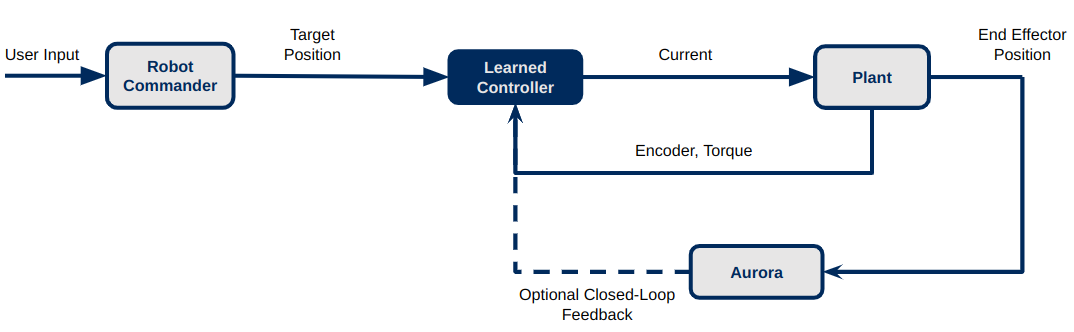
\includegraphics[width=0.9\textwidth]{images/learned_option1.png}
         \caption{Learning-based controller implementation replacing motor controller}
         \label{fig:learning_model1}
     \end{subfigure}
     \hfill
     \begin{subfigure}[b]{\textwidth}
         \centering
         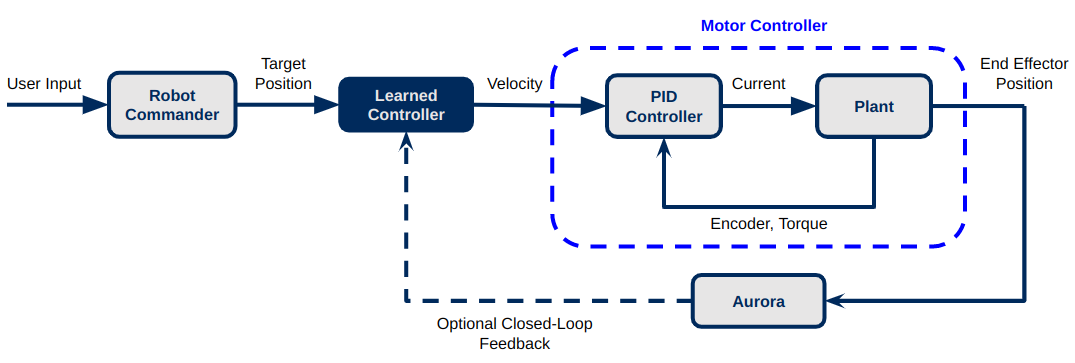
\includegraphics[width=0.9\textwidth]{images/learned_option2.png}
         \caption{Learning-based controller implementation as just the robot controller}
         \label{fig:learning_model2}
     \end{subfigure}
        \caption{Learning-based controller implementation pipeline options}
        \label{fig:learning_model_options}
\end{figure}

\paragraph{Option 1} 
In the first option (Figure \ref{fig:learning_model1}), the learned model is responsible for more aspects of control. This gives the model more flexibility in its approach to control as it has access to a lower-level control signal. However, elements of control that the PID motor controller accounts for such as limiting the change in command signals or reducing accumulated error over time are also required to be learned to achieve comparable performance. 

\paragraph{Option 2}
In the second option (Figure \ref{fig:learning_model2}), the motor controller remains in the loop. This approach has the learned controller replace one of the two baseline controllers presented in Section \ref{sec:baselines}.  This approach may be limited in accuracy as the inclusion of a PID controller restricts the system's output. 

\subsubsection{Dataloaders}
Two dataloaders were developed in order to provide an interface between the robot's data logs and the Pytorch deep learning library\footnote{https://pytorch.org/}, one designed for learning control and the other for state estimation.

\begin{figure}[H]
     \centering
     \begin{subfigure}[b]{0.8\textwidth}
         \centering
         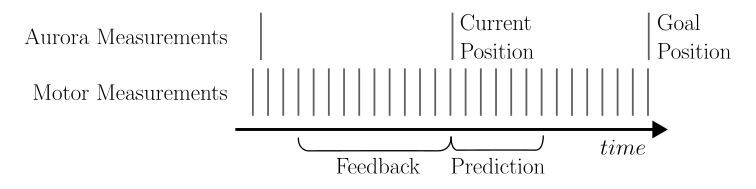
\includegraphics[width=\textwidth]{images/dataloader1.png}
         \caption{Control dataloader data representation}
         \label{fig:dataloader1}
     \end{subfigure}
     \hfill
     \begin{subfigure}[b]{0.8\textwidth}
         \centering
         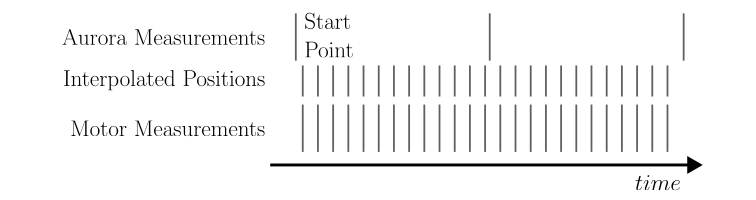
\includegraphics[width=\textwidth]{images/dataloader2.png}
         \caption{State estimation dataloader data representation}
         \label{fig:dataloader2}
     \end{subfigure}
        \caption{Representation of data loader with dataloader}
        \label{fig:dataloaders}
\end{figure}

\paragraph{The control dataloader} provides as input the robot's current ground truth position, a horizon of feedback from the motor controller, and the robot's next ground truth position. Each of these inputs is available to the robot in real time during closed-loop operation. For open-loop control, the current position input should either not be used or replaced with the output of a state estimation module. The labels provided are the next N motor commands. Figure \ref{fig:dataloader1} shows the timing breakdown of each of the provided pieces of data for this dataloader. 

\paragraph{The state estimation dataloader} provides as input the robot's starting position, and a series of feedback from the motor controller. The labels provided are an interpolation of the robot's ground truth state as measured at each motor controller feedback tick. The dataloader linearly interpolates the AURORA data to provide a state vector for every motor feedback command available. Figure \ref{fig:dataloader2} shows the timing breakdown of each of the provided pieces of data for this dataloader. 
